\documentclass[pdftex,a4paper]{scrartcl}
\usepackage{ngerman}
\usepackage[latin1]{inputenc}
\usepackage[T1]{fontenc}
\usepackage[inner=2cm,outer=2cm,top=2cm,bottom=2cm,includeheadfoot]{geometry}
\usepackage{rotating}
\usepackage{paralist}
\usepackage{url}
\usepackage{graphicx}
\setlength{\evensidemargin}{\paperwidth}
\addtolength{\evensidemargin}{-\textwidth}
\addtolength{\evensidemargin}{-2.0in}
\addtolength{\evensidemargin}{-\oddsidemargin}
\setlength{\parindent}{0pt}
%\renewcommand{\labelenumi}{\alph{enumi})}
\parskip 12pt


\usepackage{fancyhdr}
\pagestyle{fancy}
\fancyhf{}
\fancyhead[L]{Sitzungsprotokoll}
%Sitzungsdatum
\fancyhead[R]{dd.mm.jjjj}
\begin{document}

\renewcommand{\headrulewidth}{0.5pt}

\fancyfoot[C]{\thepage}
\fancyfoot[R]{\today}
\renewcommand{\footrulewidth}{0.5pt}

\begin{center}
\sc
%X-te Sitzung
\LARGE{Protokoll zur 5. Sitzung - Teil 1} \\
%Sitzungsdatum
\Large{\textbf{am 06.05.2010}} \\
%Uhrzeit
\normalsize{\textbf{um 12:00 - 16:00}}
\end{center}
%Moderator bzw Sitzungsleiter
\begin{large}\textbf{Sitzungsleiter:} Timo Michelsen\\
%Protokolant
\textbf{Protokolf"uhrer:} Daniel Twumasi\\
%Wer anwesend ist und wer nicht
\textbf{Anwesend:} Wolf Bauer, Benjamin Gr\"unebast, Volker Janz, Nico Klein, Tobias Krahn, Timo Michelsen, Sven M\"uller, Hauke Neemann, Daniel Twumasi, Thomas Vogelgesang
\newline

\end{large}
\rule{\textwidth}{0.2pt}
\rm


%~~~+++ Tagesordnungsvorstellung +++~~~
% Hier steht zun�chst die vorgeschlagene Tagesordnung f�r die Sitzung
\chapter{Tagesordnung}
 \begin{itemize}
	\item Vorstellung der Anforderungen
	\item Erstellen eines Kontextmodells
 \end{itemize}

%~~~+++ Briefing +++~~~
% Hier steht ein Briefing, sofern durchgef�hrt
\section{Anforderungen}
	\begin{itemize}
		\item Jede Gruppe hat ihre Anforderungen vorgestellt.
		 \item Diese sind im SVN unter Anforderungen zu finden.
   \end{itemize}


%~~~+++ N�chster Punkt  +++~~~ 
\section{Kontextmodell}
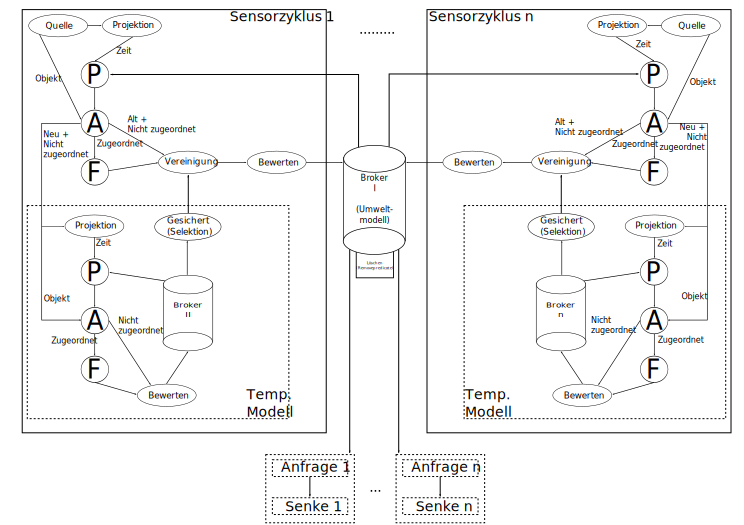
\includegraphics[scale=0.15]{Umweltmodellerschaffungszyklen.jpg}
\begin{itemize}
	\item Antreffende Daten werden mit Hilfe von Transformationsregeln verarbeitet, welche feststellen, welcher physikalische Operator f\"ur die Verarbeitung der Daten am besten geeignet ist.
	\item Der gesamte Erkennungszyklus ist n-Mal vorhanden. Einmal pro Objekttyp welcher erkannt werden soll (Auto, Schilder, Personen, etc..)
	\item Die Quelle stellen die von Simulator gelieferten Sensordaten bez\"uglich eines Objektes dar. (z.B. Autos)
	\item Die Objektverfolgung ist eingeteilt in die drei Teilschritte: P Pr\"adikation, A Assoziation (ggf. mit Gating), und F Filterung in dieser Reihenfolge.
	\item Broker 1 stellt den Broker und zugleich das Umweltmodell dar, indem nur sicher erkannte Objekte dargestellt werden.
	\item Im Broker 2 werden neu erkannte Objekte zun\"achst gespeichert. Hier erfolgt ebenfalls eine Objektverfolgung.
	\item Auf das Umweltmodell k\"onnen Anfragen vom FAZ gestellt werde. Das FAZ bekommt nur von dort seine Daten.
\end{itemize}	

\begin{itemize}
 
\item Von antreffenden Sensordaten werden Zeitstempel (Projektion) an die Pr\"adikation weitergeleitet. Die Objekte selbst werden an die Assoziation weitergeleitet. 
\item Sollte diese feststellen, dass das Objekt bereits erkannt wurde, jedoch in diesem Schritt nicht assoziert werden konnte, so wird dieses an die Bewerten \& L\"oschen Funktion weitergeleitet. Dies dient dem Zwecke der Entfernung alter Objekte, sowie der Ermittlung der Wahrscheinlichkeit, dass ein Objekt tats\"achlich existiert. Ggf. wird diese Objekt dann gel\"oscht oder an das Umweltmodell weitergeleitet. (Kann mit CEP realisiert werden, ggf. Nutzung von Metadaten)
 \item Sollte das Objekt alt und zugeordnet worden sein, wird es an die Filterung weitergegeben, danach kommt es ins Umweltmodell.
 \item Neue Objekte, welche nicht zugeordnet werden konnten, werden nach links in das tempor\"are Modell f\"ur neue Objekte  weitergeleitet und zwar das Objekt zur Assoziation und der Zeitstempel zur Pr\"adikation. 
\item Hier erfolgt analog dann ein weiterer Zyklus zur Erkennung von Objekten. Wenn Objekte hier als sicher erkannt eingestuft werden, so werden diese ins eigentliche Umweltmodell \"ubertragen.
\end{itemize}


%~~~+++ Arbeitsauftr�ge +++~~~
\section{Arbeitsauftr\"age und Fragen}
\begin{itemize}
	\item Jemand soll sich mit dem objektrelationalen Modell besch\"aftigen und Ergebnisse vorstellen. Wie werden Objekte identifiziert, verarbeitet, gejoint, etc ?
	\item Thomas stellt seine Bachelorarbeit zum Thema CEP ins Repository.
 	\item Wie funktionieren Buffer, und welche Strategien verwenden diese? (Full,...)
	\item Wird CEP f\"ur die Realiserung ben\"otigt?.
\end{itemize}

%~~~+++ N�chste Sitzung +++~~~
\section{N\"achste Sitzung}
	\begin{tabular}{|c|c|c|c|c|}
		\hline 
		Datum & Zeit & Ort & Sitzungsleiter & Protokollf"uhrer\\
		\hline 
		Tag, 10.05.2010 & 14:00 - 16:00 & OFFIS U61 & Hauke Neemann & ??	\\
		\hline
	\end{tabular}

\end{document}